\documentclass[handout]{ximera}
%handout:  for handout version with no solutions or instructor notes
%handout,instructornotes:  for instructor version with just problems and notes, no solutions
%noinstructornotes:  shows only problem and solutions

%% handout
%% space
%% newpage
%% numbers
%% nooutcomes

%I added the commands here so that I would't have to keep looking them up
%\newcommand{\RR}{\mathbb R}
%\renewcommand{\d}{\,d}
%\newcommand{\dd}[2][]{\frac{d #1}{d #2}}
%\renewcommand{\l}{\ell}
%\newcommand{\ddx}{\frac{d}{dx}}
%\everymath{\displaystyle}
%\newcommand{\dfn}{\textbf}
%\newcommand{\eval}[1]{\bigg[ #1 \bigg]}

%\begin{image}
%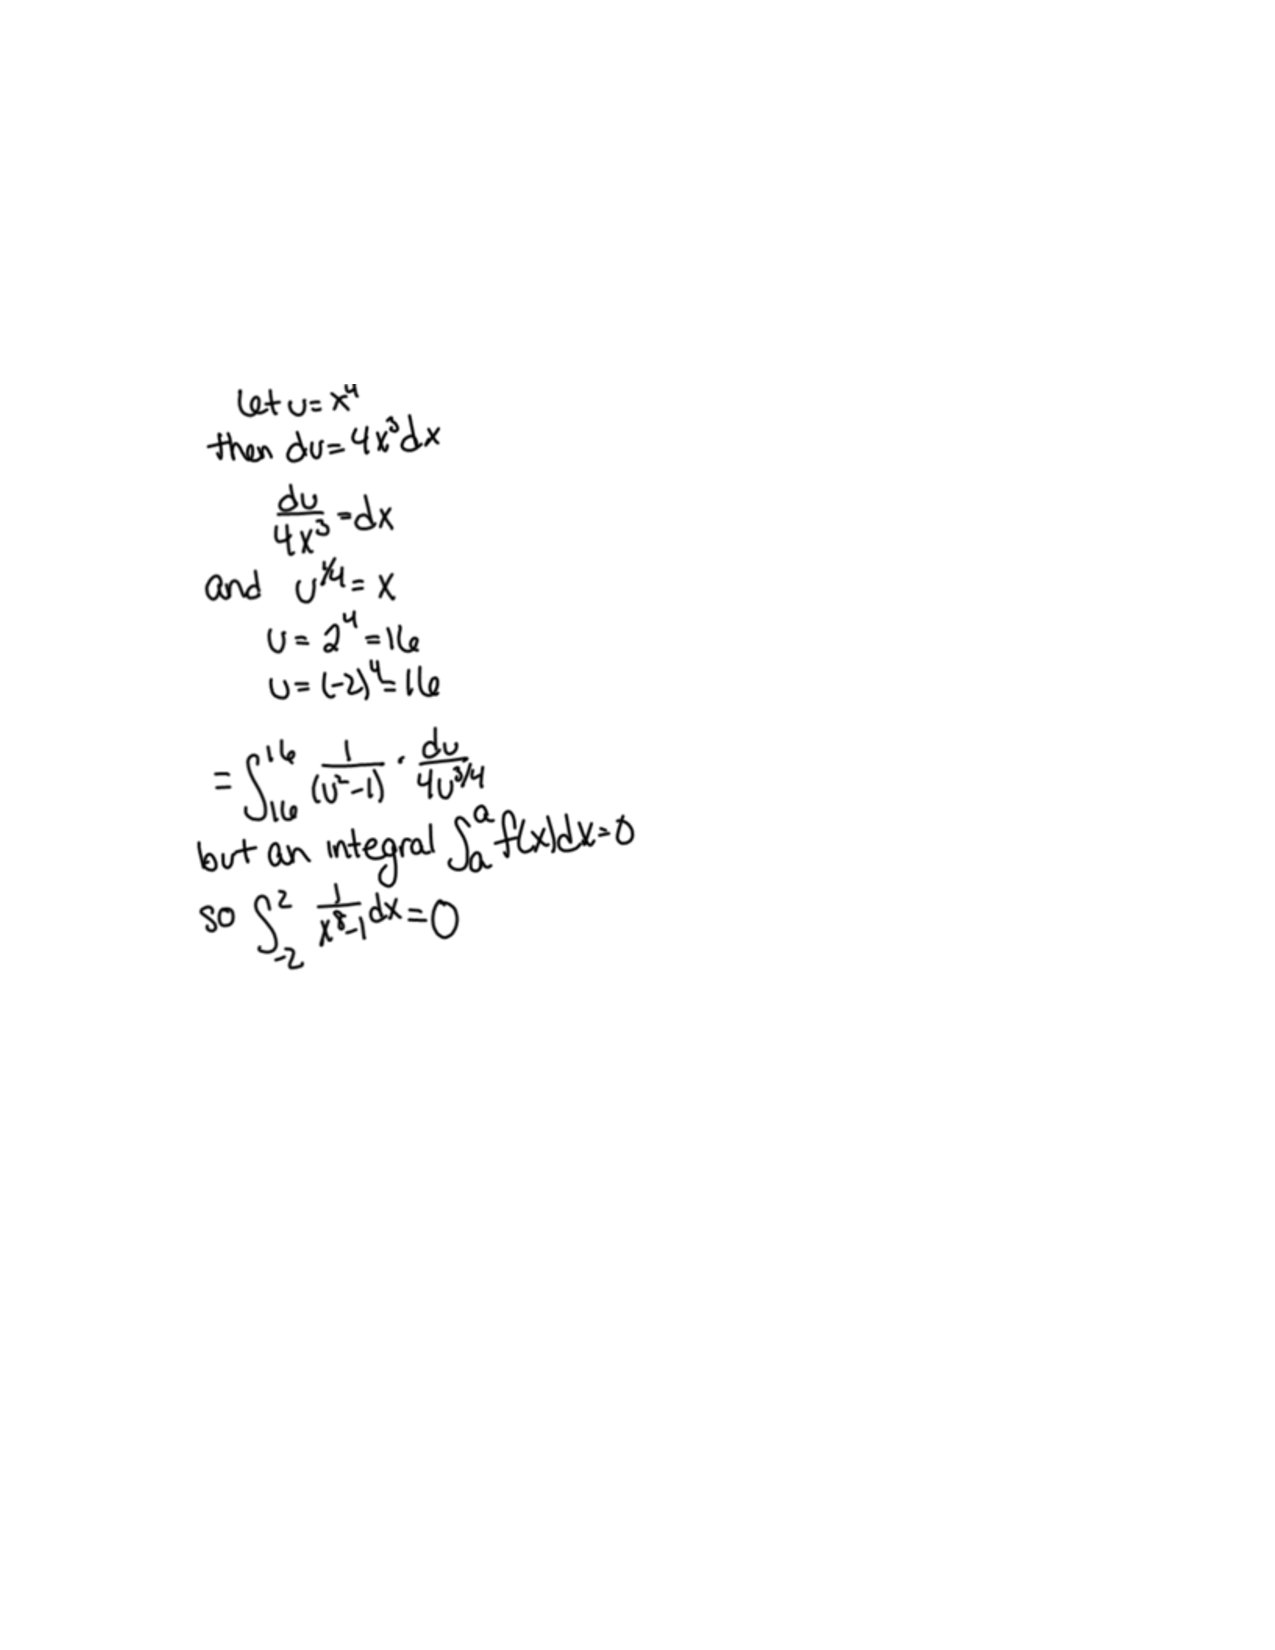
\includegraphics[trim= 170 420 250 180]{Figure1.pdf}
%\end{image}

%add a ``.'' below when used in a specific directory.
\newcommand{\RR}{\mathbb R}
\renewcommand{\d}{\,d}
\newcommand{\dd}[2][]{\frac{d #1}{d #2}}
\renewcommand{\l}{\ell}
\newcommand{\ddx}{\frac{d}{dx}}
\newcommand{\dfn}{\textbf}
\newcommand{\eval}[1]{\bigg[ #1 \bigg]}

\usepackage{multicol}

\renewenvironment{freeResponse}{
\ifhandout\setbox0\vbox\bgroup\else
\begin{trivlist}\item[\hskip \labelsep\bfseries Solution:\hspace{2ex}]
\fi}
{\ifhandout\egroup\else
\end{trivlist}
\fi} %% we can turn off input when making a master document

\title{Recitation \# 7: Exponential models and approaches to integration}  

\begin{document}
\begin{abstract}		\end{abstract}
\maketitle



\begin{comment}
\section{Warm up:}

	\begin{freeResponse}
	
	\end{freeResponse}
	
\begin{instructorNotes}

\end{instructorNotes}
\end{comment}







\section{Group work:}



%problem 1
\begin{problem}
Vitameatavegamin is a strange substance that comes in two forms.  
V-I decays at a linear rate, while V-II decays at an exponential rate.  
Both have the property that $10$ ounces will decrease to $7$ ounces in $6$ hours.  
For each of V-I and V-II, answer the following:
	\begin{enumerate}
	
	\item  If we started with $80$ ounces, how much will there be $6$ hours later?
	\begin{freeResponse}
	\dfn{V-I:}  Recall that in the linear decay model
		\[
		y(t) = -k \cdot t + y_0
		\]
	where $k$ denotes the rate of decay and $y_0$ is the initial amount.  
	We are given that $y_0 = 80oz$.  
	Clearly, we also have that
		\[
		y'(t) = -k.
		\]
	In the linear decay model, the rate of decay does not depend on the initial amount.  
	So from the given information, we have that
		\[
		-k = \frac{10oz - 7oz}{0hr - 6hr} = - \frac{1}{2}.  
		\]
	Thus, $y(t) = - \frac{1}{2} t + 80$, and therefore
		\[
		y(6) = - \frac{1}{2} (6) + 80 = 77 oz.
		\]
		
	\vskip 10pt	
		
	\dfn{V-II:}  Recall that in the exponential decay model
		\[
		y(t) = y_0 \cdot e^{-k \cdot t}
		\]
	where again $y_0 = 80oz$ is the initial amount.  
	Also notice that
		\begin{align*}
		y'(t) &= -k y_0 e^{-kt}  \\
		&= -k y(t)  \\
		\Longrightarrow &\qquad y'(0) = -k y_0.
		\end{align*}
	
	It is given that it takes $6$ hours for $10$ ounces to decrease to $7$ ounces.  
	In other words, it takes $6$ hours for $70\%$ of the substance to remain.
	So we have that
		\begin{align*}
		y(6) &= \frac{7}{10} y_0  \\
		&\Longrightarrow  \qquad  y_0 e^{-k \cdot 6} = \frac{7}{10} y_0  \\
		&\Longrightarrow  \qquad  e^{-6k} = \frac{7}{10}  \\
		&\Longrightarrow  \qquad -6k = \ln \left(\frac{7}{10} \right) = - \ln \left( \frac{10}{7} \right)  \\
		&\Longrightarrow  \qquad  k = \frac{1}{6} \ln \left( \frac{10}{7} \right).
		\end{align*}
	Thus,
		\begin{align*}
		y(6) &= 80 e^{- \frac{1}{6} \ln \left( \frac{10}{7} \right) \cdot 6}  \\
		&= 80 e^{- \ln \left( \frac{10}{7} \right)}  \\
		&= 80 \cdot \frac{7}{10} = 56oz.
		\end{align*}
	\end{freeResponse}
	
	
	
	\item  How long will it take to decrease from $15$ ounces to $7.5$ ounces?
	\begin{freeResponse}
	\dfn{V-I:}  Recall from above that $k = \frac{1}{2}$.  
	Then since $y_0$ is now $15$, we have that
		\[
		y(t) = - \frac{1}{2} t + 15.
		\]
	We want to find $t$ such that $y(t) = 7.5$.  
	So we solve
		\begin{align*}
		7.5 &= - \frac{1}{2} t + 15  \\
		- \frac{15}{2} &= - \frac{1}{2} t  \\
		t &= 15 \text{ hours}.
		\end{align*}
		
	\vskip 10pt
	
	\dfn{V-II:}  Again, since $y_0$ is now $15$, we know from above that
		\[
		y(t) = 15 e^{- \frac{1}{6} \ln \left( \frac{10}{7} \right) \cdot t}.
		\]
	We want to find $t$ such that $y(t) = 7.5 = \frac{15}{2}$.  So we solve
		\begin{align*}
		\frac{15}{2} &= 15 e^{- \frac{1}{6} \ln \left( \frac{10}{7} \right) \cdot t}  \\
		\frac{1}{2} &= e^{- \frac{1}{6} \ln \left( \frac{10}{7} \right) \cdot t}  \\
		\ln \left( \frac{1}{2} \right) &= - \frac{1}{6} \ln \left( \frac{10}{7} \right) \cdot t  \\
		\ln \left( \frac{10}{7} \right) t &= - 6 \ln \left( \frac{1}{2} \right) = 6 \ln 2  \\
		t &= \frac{6 \ln 2}{\ln \left( \frac{10}{7} \right) } \text{ hours}.
		\end{align*}
	\end{freeResponse}
	
	\end{enumerate}
	
\end{problem}

\begin{instructorNotes}
The issue is to compare and contrast linear and exponential decay.  
To solve, it is implicit to find the slope (I) and $k$ (II) first before proceeding (this may need a prompt).
\end{instructorNotes}








%problem 2
\begin{problem}
Evaluate
	\[
	\int \frac{5x^3 - 6x + 2}{x-5} \d x.
	\]
	\begin{freeResponse}
	When integrating a rational function (i.e., a fraction of polynomials) where the degree of the numerator is greater than or equal to the degree of the denominator, we need to use long division to simplify the expression.  
	
	\begin{image}
	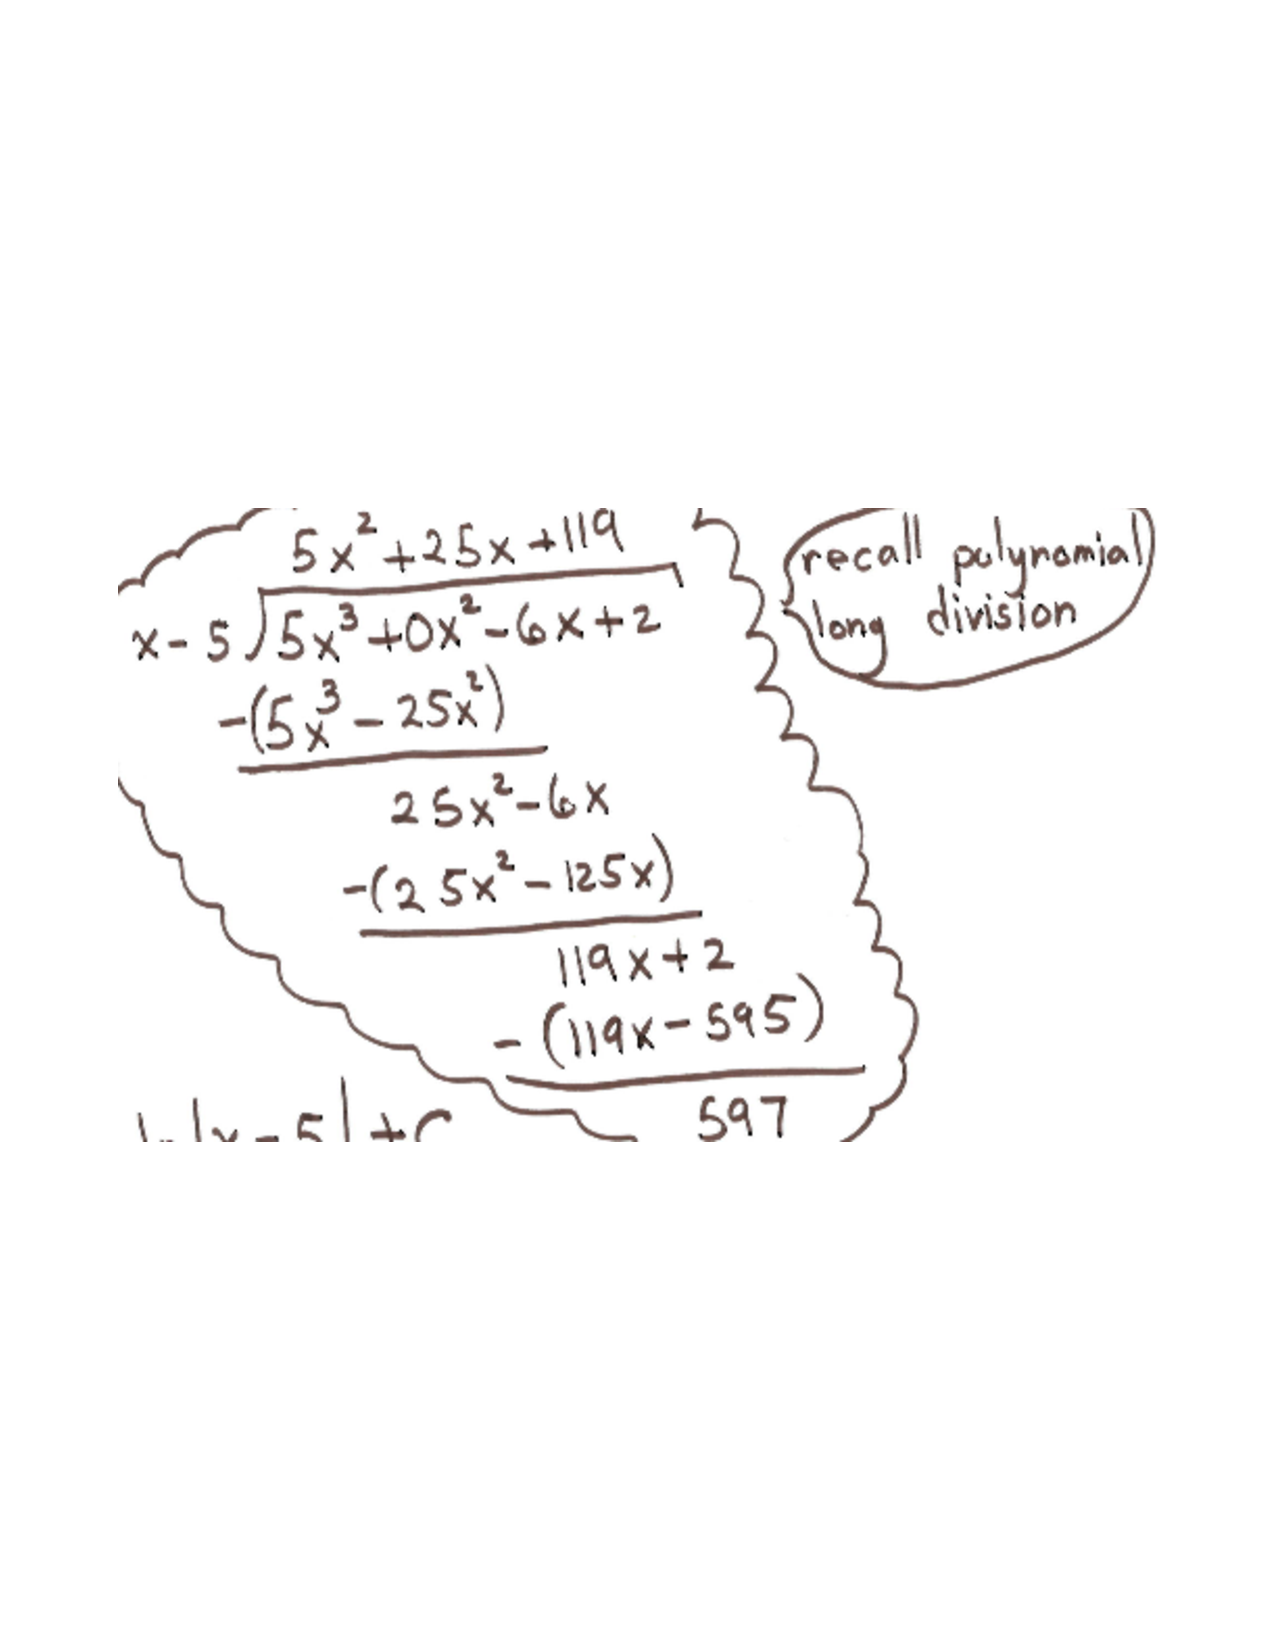
\includegraphics[trim= 170 220 250 250, scale=0.7]{Figure7-1-1.pdf}
	\end{image}
	
	So
		\[
		\frac{5x^3 - 6x + 2}{x-5} = 5x^2 + 25x + 119 + \frac{597}{x-5}
		\]
	and therefore
		\begin{align*}
		\int \frac{5x^3 - 6x + 2}{x-5} \d x &= \int \left( 5x^2 + 25x + 119 + \frac{597}{x-5} \right) \d x  \\
		&= \frac{5}{3} x^3 + \frac{25}{2} x^2 + 119x + 597 \int \frac{1}{x-5} \d x.
		\end{align*}
	To evaluate
		\[
		\int \frac{1}{x-5} \d x
		\]
	we technically should perform a substitution.  
	But since $\ddx (x-5) = 1$, we can treat $x-5$ as a variable during integration.  
	Thus
		\[
		\int \frac{1}{x-5} \d x = \ln |x-5|
		\]
	and therefore
		\[
		\int \frac{5x^3 - 6x + 2}{x-5} \d x = \frac{5}{3} x^3 + \frac{25}{2} x^2 + 119x + 597 \ln |x-5| + C.
		\]
	\end{freeResponse}
	
\end{problem}

\begin{instructorNotes}
Each of problems \#1 through \#4 presents a different aspect that is covered in Section 7.1.  
This problem (\# 1) requires long division.  
\end{instructorNotes}







%problem 3
\begin{problem}
Evaluate
	\[
	\int \frac{5}{3^{2x} + 3^{-2x}} \d x.
	\]
	\begin{freeResponse}
		\begin{align*}
		\int \frac{5}{3^{2x} + 3^{-2x}} \d x &= \int \frac{5}{3^{2x} + 3^{-2x}} \cdot \frac{3^{2x}}{3^{2x}} \d x  \\
		&= \int \frac{5 \cdot 3^{2x}}{\left( 3^{2x} \right)^2 + 1} \d x .
		\end{align*}
	Now, let 
		\[
		u = 3^{2x}.
		\]  
	Then 
		\[
		\d u = 2 \cdot 3^{2x} \cdot \ln (3) \d x
		\]
	and so
		\[
		\d x = \frac{1}{2 \cdot 3^{2x} \cdot \ln (3)} \d u.
		\]
	Thus
		\begin{align*}
		\int \frac{5}{3^{2x} + 3^{-2x}} \d x &= \int \frac{5}{u^2 + 1} \cdot \frac{1}{2\ln(3)} \d u  \\
		&= \frac{5}{2\ln(3)} \arctan(u) + C  \\
		&= \frac{5}{2\ln(3)} \arctan \left( 3^{2x} \right) + C.
		\end{align*}
	\end{freeResponse}
		
\end{problem}

\begin{instructorNotes}
Students are likely to have forgotten $\ddx \left( C^x \right)$ for $C \neq e$.
\end{instructorNotes}







%problem 4
\begin{problem}
Evaluate the following integrals
	\begin{enumerate}
	
	\item  $\int \frac{\cos x}{1 + \sin x} \d x$
	\begin{freeResponse}
	Let $u=1+\sin x$.  Then $\d u = \cos x \d x$, and so
		\begin{align*}
		\int \frac{\cos x}{1 + \sin x} \d x &= \int \frac{1}{u} \d u  \\
		&= \ln|u| + C  \\
		&= \ln (1 + \sin(x) ) + C.
		\end{align*}
	\end{freeResponse}
	
	
	
	\item  $ \int \frac{1}{\sin x - 1} \d x$
	\begin{freeResponse}
		\begin{align*}
		\int \frac{1}{\sin x - 1} \d x &= \int \frac{1}{\sin x - 1} \cdot \frac{\sin x + 1}{\sin x + 1} \d x  \qquad  {\color{red}\text{since } \frac{\sin x + 1}{\sin x + 1} = 1}\\
		&= \int \frac{\sin x + 1}{\sin^2 x - 1} \d x  \\
		&= \int \frac{\sin x + 1}{-\cos^2 x} \d x		\qquad	{\color{red}\text{since } \cos^2 x + \sin^2 x = 1}  \\
		&= \int \frac{-\sin x}{\cos^2 x} \d x - \int \frac{1}{\cos^2 x} \d x.
		\end{align*}
	Now we split up and compute these two integrals separately.
		\begin{align*}
		\int \frac{-\sin x}{\cos x} \d x &= \int \frac{1}{u^2} \d u	\qquad	{\color{red} \text{where } u = \cos x, \d u = - \sin x \d x}  \\
		&= - \frac{1}{u} + C = \frac{-1}{\cos x} + C.
		\end{align*}
	Also,
		\[
		\int \frac{1}{\cos^2 x} \d x = \int \sec^2 x \d x = \tan x + C.
		\]
	So, we finally have that
		\[
		\int \frac{1}{\sin x - 1} \d x = \frac{-1}{\cos x} - \tan x + C.
		\]
	\end{freeResponse}
	
	\end{enumerate}

\end{problem}

\begin{instructorNotes}
The two integrals in this problem look similar, but they require very different strategies in order to rewrite them as ``basic" integrals.
\end{instructorNotes}







%problem 5
\begin{problem}
Evaluate the following integrals
	\begin{enumerate}
	
	\item  $ \int \frac{13}{\sqrt{12x - x^2 - 20}} \d x$
	\begin{freeResponse}
	First notice that by completing the square, we have that
		\begin{align*}
		12x - x^2 - 20 &= -(x^2 - 12x) - 20  \\
		&= -(x^2 - 12x + {\color{red}36}) - 20 + {\color{red}36}  \\
		&= 16 - (x-6)^2  \\
		&= 16 \left( 1 - \frac{(x-6)^2}{16} \right)  \\
		&= 16 \left( 1 - \left( \frac{x-6}{4} \right)^2 \right).
		\end{align*}
	Then
		\begin{align*}
		\int \frac{13}{\sqrt{12x - x^2 - 20}} \d x &= \int \frac{13}{\sqrt{16 \left( 1 - \left( \frac{x-6}{4} \right)^2 \right)}} \d x  \\
		&= \frac{13}{4} \int \frac{1}{\sqrt{1 - \left( \frac{x-6}{4} \right)^2}} \d x.
		\end{align*}
	
	Let
		\[
		u = \frac{x-6}{4} = \frac{1}{4} (x-6).
		\]
	Then
		\[
		\d u = \frac{1}{4} \d x		\qquad	\Longrightarrow		\qquad	4 \d u = \d x.
		\]
	Finally, we have that
		\begin{align*}
		\int \frac{13}{\sqrt{12x - x^2 - 20}} \d x &= 13 \int \frac{1}{\sqrt{1-u^2}} \d u  \\
		&= 13 \arcsin(u) + C  \\
		&= 13 \arcsin \left( \frac{x-6}{4} \right) + C.
		\end{align*}
	\end{freeResponse}
	
	
	
	\item  $\int \frac{13x^3}{\sqrt{12x^6 - x^8 - 20x^4}} \d x$
	\begin{freeResponse}
		\begin{align*}
		\int \frac{13x^3}{\sqrt{12x^6 - x^8 - 20x^4}} \d x &= \int \frac{13x^3}{\sqrt{x^4} \cdot \sqrt{12x^2-x^4-20}} \d x  \\
		&= \int \frac{13x}{\sqrt{12x^2-x^4-20}} \d x  \\
		&= \frac{1}{2} \int \frac{13}{\sqrt{12u-u^2-20}} \d u	\qquad	{\color{red} \text{Let }u=x^2, \d u = 2 x \d x }  \\
		&= \frac{1}{2} \left( 13 \arcsin \left( \frac{u-6}{4} \right) \right) + C	\qquad	{\color{red}\text{from part (a)}}  \\
		&= \frac{13}{2} \arcsin \left( \frac{x^2 - 6}{4} \right) + C.
		\end{align*}
	\end{freeResponse}
	
	
	
	\item  $\int \frac{13e^{4x}}{\sqrt{ 12e^{6x} - e^{8x} - 20e^{4x} }} \d x$
	\begin{freeResponse}
		\begin{align*}
		\int \frac{13e^{4x}}{\sqrt{ 12e^{6x} - e^{8x} - 20e^{4x} }} \d x &= \int \frac{13e^{4x}}{\sqrt{e^{4x}} \cdot \sqrt{12e^{2x} - e^{4x} - 20}} \d x  \\
		&= \int \frac{13e^{2x}}{\sqrt{12e^{2x} - e^{4x} - 20}} \d x  \\
		&= \frac{1}{2} \int \frac{13}{\sqrt{12u - u^2 - 20}} \d u		\qquad	{\color{red} \text{where } u=e^{2x}, \d u = 2e^{2x} \d x}  \\
		&= \frac{1}{2} \left( 13 \arcsin \left( \frac{u-6}{4} \right) \right) + C	\qquad 	{\color{red}\text{from part (a)}}  \\
		&= \frac{13}{2} \arcsin \left( \frac{e^{2x}-6}{4} \right) + C.
		\end{align*}
	\end{freeResponse}
	
	\end{enumerate}

\end{problem}

\begin{instructorNotes}
Part (a) of this problem involves completing the square.  
Parts (b) and (c) both require you to factor out a common factor, as well as substitute, to get the same integral as in part (a).  
You may want to do part (a) as a whole class, and then split parts (b) and (c) between the groups.  
Then let them present the substitution which returns part (a).  
\end{instructorNotes}





















	
	
	
	
	
	
	
	
	

	










								
				
				
	














\end{document} 


















